
\cvsection{Education}

\cvevent{Ph.D.\ in Robotics}{Georgia Institute of Technology}{August 2011 -- July 2017}{}
Advised by: C. Karen Liu, Aaron Ames, and Mike Stilman

\divider

\cvevent{B.Sc.\ in Aerospace Engineering}{University of Illinois at Urbana-Champaign}{August 2007 -- May 2011}{}

\cvsection{Projects}

\cvachievement{\href{https://github.com/osrf/rmf_core}{
\includegraphics[width=\linewidth]{ros-health.png}}}{\href{https://github.com/osrf/rmf_core}{RMF}}{Designer and maintainer}

\divider

\cvachievement{\href{https://github.com/osrf/soss}{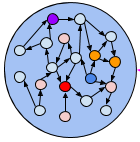
\includegraphics[width=\linewidth]{soss_bubbles.png}}}{\href{https://github.com/osrf/soss}{SOSS}}{Co-designer and co-maintainer}

\divider

\cvachievement{\href{https://github.com/dartsim/dart}{
\includegraphics[width=\linewidth]{dart_logo.jpg}}}{\href{https://github.com/dartsim/dart}{Dynamic Anim. and Robotics Toolkit}}{Co-designer and co-maintainer}

\divider

\cvachievement{\href{https://bitbucket.org/ignitionrobotics/ign-physics/}{
\includegraphics[width=\linewidth]{ignition_logo.png}}}{\href{https://bitbucket.org/ignitionrobotics/ign-physics/}{Ignition Physics}}{Designer and co-maintainer}

\divider

\cvachievement{\href{http://gazebosim.org/}{
\includegraphics[width=\linewidth]{gazebo.png}}}{\href{http://gazebosim.org/}{Gazebo}}{Contributor and co-maintainer}

\divider

\cvachievement{\href{https://www.ros.org/}{
\includegraphics[width=\linewidth]{ros1.png}}}{\href{https://www.ros.org/}{ROS1}}{Contributor}

\divider

\cvachievement{\href{https://index.ros.org/doc/ros2/}{
\includegraphics[width=\linewidth]{ros2.png}}}{\href{https://index.ros.org/doc/ros2/}{ROS2}}{Contributor}

\cvsection{Robotics Interests}
\cvtag{Planning}
\cvtag{Locomanipulation}
\cvtag{Dynamics}
\cvtag{Controls}
\cvtag{Teleoperation}

\cvsection{Design Focus}
\cvtag{Reliability}
\cvtag{Robustness}
\cvtag{Maintainability}
\cvtag{Visualization}
\cvtag{User-friendliness}

\cvsection{Languages}

\cvtag{C++}
\cvtag{Python}
\cvtag{Java}
\cvtag{Matlab}

%% Yeah I didn't spend too much time making all the 
%% spacing consistent... sorry. Use \smallskip, \medskip, 
%% \bigskip, \vpsace etc to make ajustments.
\medskip
